%\documentclass[hyperref={pdfpagelabels=false},slidetop,9pt]{beamer}
\documentclass[slidetop,8pt]{beamer}
\usepackage[T1]{fontenc}
\usepackage[utf8]{inputenc}
\newcommand{\id}{54}
\newcommand{\nom}{Liaisons mécaniques}
\newcommand{\sequence}{04}
\newcommand{\num}{01}
\newcommand{\type}{TP}
\newcommand{\descrip}{Modélisation d'un solide. Comportement des liaisons mécaniques. Modéliser les mécanismes du laboratoire par un schéma cinématique, paramétré.}
\newcommand{\competences}{A3-C4: Analyse d'architecture et de comportement \\ &  Mod1-C1: Isolement d'un solide ou d'un système de solides \\ &  Mod2-C10-1: Modèle de solide indéformable \\ &  Mod2-C11: Modélisation géométrique et cinématique des mouvements entre solides indéformables \\ &  Mod2-C12: Modélisation cinématique des liaisons entre solides \\ &  Mod2-C15: Modélisation des actions mécaniques \\ &  Rés-C6: Utilisation d'un solveur ou d'un logiciel multi physique \\ &  Com1-C1: Différents descripteurs introduits dans le programme \\ &  Com2-C4: Outils de communication}
\newcommand{\nbcomp}{9}
\newcommand{\systemes}{Plateforme Stewart}
\newcommand{\systemessansaccent}{Plateforme Stewart}
\newcommand{\ilot}{2}
\newcommand{\ilotstr}{02}
\newcommand{\dossierilot}{\detokenize{Ilot_02 Plateforme Stewart}}
\newcommand{\imageun}{Plateforme}

\newcommand{\urlsysteme}{\href{https://www.costadoat.fr/systeme/57}{Ressources système}}
\newcommand{\matlabsimscape}{\href{https://github.com/Costadoat/Sciences-Ingenieur/raw/master/Systemes/Plateforme Stewart/Plateforme_Stewart_Simscape.zip}{Modèle Simscape}}
\newcommand{\solidworks}{\href{https://github.com/Costadoat/Sciences-Ingenieur/raw/master/Systemes/Plateforme Stewart/Plateforme_Stewart_Solidworks.zip}{Modèle Solidworks}}
\newcommand{\edrawings}{\href{https://github.com/Costadoat/Sciences-Ingenieur/raw/master/Systemes/Plateforme Stewart/Plateforme_Stewart.EASM}{Modèle eDrawings}}
\newcommand{\test}{Stewart_param1}
\newcommand{\testi}{Stewart_param2}
\newcommand{\testii}{Stewart_param3}
\newcommand{\testiii}{Stewart_param4}
\newcommand{\testiiii}{Stewart_euler}
\usepackage{etex}
\usepackage{tikz}
\usepackage[european]{circuitikz}
\usepackage{pgf}
\usepackage[all]{xy}
\usepackage{pgfpages}
\usepackage{graphbox}
\usepackage{pdfpages}
\usepackage[adobe-utopia]{mathdesign}
\usepackage{ifthen}
\usepackage{cancel}
\usepackage{framed}
\usepackage{subfig}
\usepackage{tabularx}
\usepackage{setspace}
\usepackage{soul}
\usepackage{schemabloc}
\usepackage{eqnarray}
\usepackage[dot, phantomtext]{dashundergaps}
\usepackage{media9}
\usepackage{multimedia}
\usepackage{textcomp}

\author{Renaud Costadoat}
\institute{Lycée Dorian}

\usepackage{multido}
\usepackage{multirow}
\usepackage{multicol} % Portions de texte en colonnes
\usepackage{flafter}%floatants après la référence

\usepackage{color}
\usepackage{xcolor}
\usepackage{colortbl}

\usepackage[gen]{eurosym}
\usepackage{tikz}
%\usepackage{pstricks,pst-node,pst-tree,pst-solides3d}
\usepackage{lmodern}
\usepackage[francais]{babel}
\usepackage{pslatex}
\usetheme{renaud}
\usepackage{times}
\usepackage{amsmath}
\usepackage{verbatim}
\usepackage{moreverb}
%\usetikzlibrary{arrows,shapes}
\usepackage{graphicx}
\usepackage{psfrag}
\usepackage{wrapfig}
\usepackage{etoolbox}

\definecolor{gris25}{gray}{0.75}
\definecolor{bleu}{RGB}{18,33,98}
\definecolor{bleuf}{RGB}{42,94,171}
\definecolor{bleuc}{RGB}{231,239,247}
\definecolor{rougef}{RGB}{185,18,27}
\definecolor{rougec}{RGB}{255,188,204}%255,230,231
\definecolor{vertf}{RGB}{103,126,82}
\definecolor{vertc}{RGB}{220,255,191}

\setlength\parindent{24pt}
\parskip 7.2pt
\parindent 8pt

\newenvironment{rem}[1][\hsize]%
{%
    \def\FrameCommand
   {%
\rotatebox{90}{\textit{\textsf{Remarque}}} 
       {\color{bleuf}\vrule width 3pt}%
       \hspace{0pt}%must no space.
       \fboxsep=\FrameSep\colorbox{bleuc}%
  }%
    \MakeFramed{\hsize#1\advance\hsize-\width\FrameRestore}%
}%
{\endMakeFramed}%


\newenvironment{savoir}[1][\hsize]%
{%
    \def\FrameCommand
    {%
\rotatebox{90}{\textit{\textsf{Savoir}}} 
        {\color{bleuf}\vrule width 3pt}%
        \hspace{0pt}%must no space.
        \fboxsep=\FrameSep\colorbox{bleuc}%
    }%
    \MakeFramed{\hsize#1\advance\hsize-\width\FrameRestore}%
}%
{\endMakeFramed}%

\newenvironment{prob}[1][\hsize]%
{%
    \def\FrameCommand%
    {%
\rotatebox{90}{\textit{\textsf{Problematique}}} 
        {\color{rougef}\vrule width 3pt}%
        \hspace{0pt}%must no space.
        \fboxsep=\FrameSep\colorbox{rougec}%
    }%
    \MakeFramed{\hsize#1\advance\hsize-\width\FrameRestore}%
}%
{\endMakeFramed}%

\newenvironment{obj}[1][\hsize]%
{%
    \def\FrameCommand%
    {%
\rotatebox{90}{\textit{\textsf{Objectif}}} 
        {\color{vertf}\vrule width 3pt}%
        \hspace{0pt}%must no space.
        \fboxsep=\FrameSep\colorbox{vertc}%
    }%
    \MakeFramed{\hsize#1\advance\hsize-\width\FrameRestore}%
}%
{\endMakeFramed}%

\newenvironment{defi}[1][\hsize]%
{%
    \def\FrameCommand%
    {%
\rotatebox{90}{\textit{\textsf{Definition}}} 
        {\color{bleuf}\vrule width 3pt}%
        \hspace{0pt}%must no space.
        \fboxsep=\FrameSep\colorbox{rougec}%
    }%
    \MakeFramed{\hsize#1\advance\hsize-\width\FrameRestore}%
}%
{\endMakeFramed}%


\newenvironment{hypo}[1][\hsize]%
{%
    \def\FrameCommand%
    {%
\rotatebox{90}{\textit{\textsf{Hypothèse\\}}} 
        {\color{bleuf}\vrule width 3pt}%
        \hspace{0pt}%must no space.
        \fboxsep=\FrameSep\colorbox{bleuc}%
    }%
    \MakeFramed{\hsize#1\advance\hsize-\width\FrameRestore}%
}%
{\endMakeFramed}%


\newenvironment{prop}[1][\hsize]%
{%
    \def\FrameCommand%
    {%
\rotatebox{90}{\textit{\textsf{Propriété}}} 
        {\color{bleuf}\vrule width 3pt}%
        \hspace{0pt}%must no space.
        \fboxsep=\FrameSep\colorbox{bleuc}%
    }%
    \MakeFramed{\hsize#1\advance\hsize-\width\FrameRestore}%
}%
{\endMakeFramed}%

\newenvironment{props}[1][\hsize]%
{%
    \def\FrameCommand%
    {%
\rotatebox{90}{\textit{\textsf{Propriétés}}} 
        {\color{bleuf}\vrule width 3pt}%
        \hspace{0pt}%must no space.
        \fboxsep=\FrameSep\colorbox{bleuc}%
    }%
    \MakeFramed{\hsize#1\advance\hsize-\width\FrameRestore}%
}%
{\endMakeFramed}%

\newenvironment{exemple}[1][\hsize]%
{%
    \def\FrameCommand%
    {%
\rotatebox{90}{\textit{\textsf{Exemple}}} 
        {\color{vertf}\vrule width 3pt}%
        \hspace{0pt}%must no space.
        \fboxsep=\FrameSep\colorbox{vertc}%
    }%
    \MakeFramed{\hsize#1\advance\hsize-\width\FrameRestore}%
}%
{\endMakeFramed}%

\newenvironment{resultat}[1][\hsize]%
{%
    \def\FrameCommand%
    {%
\rotatebox{90}{\textit{\textsf{Résultat}}} 
        {\color{rougef}\vrule width 3pt}%
%        {\color{bleuf}\vrule width 3pt}%
        \hspace{0pt}%must no space.
        \fboxsep=\FrameSep\colorbox{rougec}%
    }%
    \MakeFramed{\hsize#1\advance\hsize-\width\FrameRestore}%
}%
{\endMakeFramed}%

\newenvironment{methode}[1][\hsize]%
{%
    \def\FrameCommand%
    {%
\rotatebox{90}{\textit{\textsf{Méthode\\}}} 
        {\color{rougef}\vrule width 3pt}%
        \hspace{0pt}%must no space.
        \fboxsep=\FrameSep\colorbox{rougec}%
    }%
    \MakeFramed{\hsize#1\advance\hsize-\width\FrameRestore}%
}%
{\endMakeFramed}%

\newenvironment{theo}[1][\hsize]%
{%
    \def\FrameCommand%
    {%
\rotatebox{90}{\textit{\textsf{Théorème\\}}} 
        {\color{rougef}\vrule width 3pt}%
        \hspace{0pt}%must no space.
        \fboxsep=\FrameSep\colorbox{rougec}%
    }%
    \MakeFramed{\hsize#1\advance\hsize-\width\FrameRestore}%
}%
{\endMakeFramed}%

\newenvironment{warn}[1][\hsize]%
{%
    \def\FrameCommand%
    {%
\rotatebox{90}{\textit{\textsf{Attention\\}}} 
        {\color{rougef}\vrule width 3pt}%
        \hspace{0pt}%must no space.
        \fboxsep=\FrameSep\colorbox{rougec}%
    }%
    \MakeFramed{\hsize#1\advance\hsize-\width\FrameRestore}%
}%
{\endMakeFramed}%

% \usepackage{pstricks}
%\usepackage{minitoc}
% \setcounter{minitocdepth}{4}

\setcounter{tocdepth}{2}

% \mtcselectlanguage{french} 

%\usepackage{draftcopy}% "Brouillon"
% \usepackage{floatflt}
\usepackage{psfrag}
%\usepackage{listings} % Permet d'insérer du code de programmation
\renewcommand{\baselinestretch}{1.2}

% Changer la num�rotation des figures :
% ------------------------------------
% \makeatletter
% \renewcommand{\thefigure}{\ifnum \c@section>\z@ \thesection.\fi
%  \@arabic\c@figure}
% \@addtoreset{figure}{section}
% \makeatother
 


%%%%%%%%%%%%
% Définition des vecteurs %
%%%%%%%%%%%%
 \newcommand{\vect}[1]{\overrightarrow{#1}}

%%%%%%%%%%%%
% Définition des torseusr %
%%%%%%%%%%%%

 \newcommand{\torseur}[1]{%
\left\{{#1}\right\}
}

\newcommand{\torseurcin}[3]{%
\left\{\mathcal{#1} \left(#2/#3 \right) \right\}
}

\newcommand{\torseurstat}[3]{%
\left\{\mathcal{#1} \left(#2\rightarrow #3 \right) \right\}
}

 \newcommand{\torseurc}[8]{%
%\left\{#1 \right\}=
\left\{
{#1}
\right\}
 = 
\left\{%
\begin{array}{cc}%
{#2} & {#5}\\%
{#3} & {#6}\\%
{#4} & {#7}\\%
\end{array}%
\right\}_{#8}%
}

 \newcommand{\torseurcol}[7]{
\left\{%
\begin{array}{cc}%
{#1} & {#4}\\%
{#2} & {#5}\\%
{#3} & {#6}\\%
\end{array}%
\right\}_{#7}%
}

 \newcommand{\torseurl}[3]{%
%\left\{\mathcal{#1}\right\}_{#2}=%
\left\{%
\begin{array}{l}%
{#1} \\%
{#2} %
\end{array}%
\right\}_{#3}%
}

 \newcommand{\vectv}[3]{%
\vect{V\left( {#1} \in {#2}/{#3}\right)}
}


\newcommand{\vectf}[2]{%
\vect{R\left( {#1} \rightarrow {#2}\right)}
}

\newcommand{\vectm}[3]{%
\vect{\mathcal{M}\left( {#1}, {#2} \rightarrow {#3}\right)}
}


 \newcommand{\vectg}[3]{%
\vect{\Gamma \left( {#1} \in {#2}/{#3}\right)}
}

 \newcommand{\vecto}[2]{%
\vect{\Omega\left( {#1}/{#2}\right)}
}

\newcommand{\reponse}[1][4]
{
\multido{}{#1}
{
\begin{center}
\makebox[0.9\linewidth]{\dotfill} \end{center}
}}


% }$$\left\{\mathcal{#1} \right\}_{#2} =%
% \left\{%
% \begin{array}{c}%
%  #3 \\%
%  #4 %
% \end{array}%
% \right\}_{#5}}


%  ------------------------------------------
% | Modification du formatage des sections : | 
%  ------------------------------------------

% Grands titres :
% ---------------

\newcommand{\titre}[1]{%
\begin{center}
      \bigskip
      \rule{\textwidth}{1pt}
      \par\vspace{0.1cm}
      
      \textbf{\large #1}
      \par\rule{\textwidth}{1pt}
    \end{center}
    \bigskip
  }

% Supprime le numéro du chapitre dans la numérotation des sections:
% -----------------------------------------------------------------
\makeatletter
\renewcommand{\thesection}{\@arabic\c@section}
\makeatother


% \titleformat{\chapter}[display]
% {\normalfont\Large\filcenter}
% {}
% {1pc}
% {\titlerule[1pt]
%   \vspace{1pc}%
%   \Huge}[\vspace{1ex}%
% \titlerule]


%%%% Chapitres Comme PY Pechard %%%%%%%%%
% numéro du chapitre
\DeclareFixedFont{\chapnumfont}{OT1}{phv}{b}{n}{80pt}
% pour le mot " Chapitre "
\DeclareFixedFont{\chapchapfont}{OT1}{phv}{m}{it}{40pt}
% pour le titre
\DeclareFixedFont{\chaptitfont}{T1}{phv}{b}{n}{25pt}

\definecolor{gris}{gray}{0.75}
\setbeamertemplate{section in toc}[sections numbered]

\newlength{\RoundedBoxWidth}
\newsavebox{\GrayRoundedBox}
\newenvironment{GrayBox}[1][\dimexpr\textwidth-4.5ex]%
   {\setlength{\RoundedBoxWidth}{\dimexpr#1}
    \begin{lrbox}{\GrayRoundedBox}
       \begin{minipage}{\RoundedBoxWidth}}%
   {   \end{minipage}
    \end{lrbox}
    \begin{center}
    \begin{tikzpicture}%
       \draw node[draw=bleuf,fill=bleuc,rounded corners,%
             inner sep=2ex,text width=\RoundedBoxWidth]%
             {\usebox{\GrayRoundedBox}};
    \end{tikzpicture}
    \end{center}}
    
\ifdef{\prive}{\pgfpagesuselayout{2 on 1}[a4paper,border shrink=0mm]}
\ifdef{\prive}{\setbeamertemplate{navigation symbols}{}}
\setbeamertemplate{itemize item}[ball]
%\setbeamertemplate{blocks}[rounded]%[shadow=true]
\setbeamercolor{block title}{fg=white,bg=grisf}        % titre block normal 
\setbeamercolor{block body}{fg=grisf,bg=grisc!50}      % corps block normal
\setbeamercolor{block body alerted}{fg=white,bg=warning}   % idem pour un block alerte

\title{\nom}
\date{S\sequence \ - \type\num}

\begin{document}
\shorthandoff{:!}
\bibliographystyle{abbrvnat-fr}

\usebackgroundtemplate%
{%
    \centering
\includegraphics[width=\paperwidth]{../../img/fond2}%
}

{
\setbeamertemplate{navigation symbols}{}
\setbeamertemplate{headline}[pagetitre]
\setbeamertemplate{footline}[pagetitre]
\usebackgroundtemplate{\centering
\includegraphics[width=\paperwidth]{../../img/fond}}
\frame{\titlepage}
}



\section{Le dessin technique}

{\frame{
\frametitle{Dessin technique}

\begin{obj}
\begin{itemize}
 \item Le dessin technique ou dessin industriel, est destiné à la communication technique et la conception.
 \item Il faut connaître un ensemble de règles pour représenter des objets associées à des codes de représentation que l'on doit savoir lire pour comprendre l'architecture et le fonctionnement d'un système.
\end{itemize}
\end{obj}
}}

{\frame{
\frametitle{Types de dessin technique}

\begin{itemize}
 \item Le schéma,
 \item Le dessin d'ensemble: \textit{Systèmes constitués de divers éléments},
 \item Le dessin de définition: \textit{Représentation d'une pièce}.
\end{itemize}

\vfill

\begin{minipage}{0.3\linewidth}
 \centering 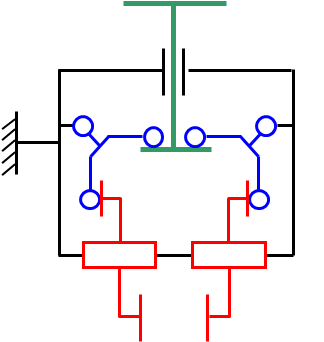
\includegraphics[width=0.8\linewidth]{img/Image5}
\end{minipage}
\hfill
\begin{minipage}{0.3\linewidth}
 \centering 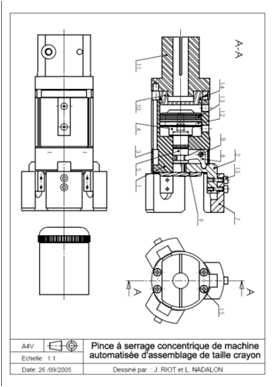
\includegraphics[width=0.7\linewidth]{img/Image3}
\end{minipage}
\hfill
\begin{minipage}{0.3\linewidth}
 \centering 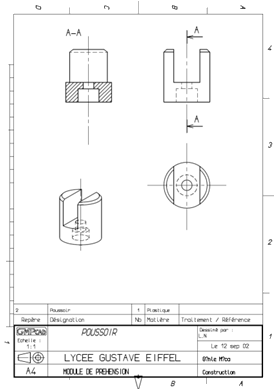
\includegraphics[width=0.7\linewidth]{img/Image4}
\end{minipage}
}}


{\frame{
\frametitle{Le cartouche}

Le cartouche contient:
\begin{itemize}
 \item Le nom de la pièce ou du mécanisme
 \item L'échelle, le format, et le symbole de disposition des vues
 \item Le nom du dessinateur et la date 
 \item un ensemble de données destinées à l'archivage du document
\end{itemize}

\vfill

\begin{minipage}{0.9\linewidth}
 \centering 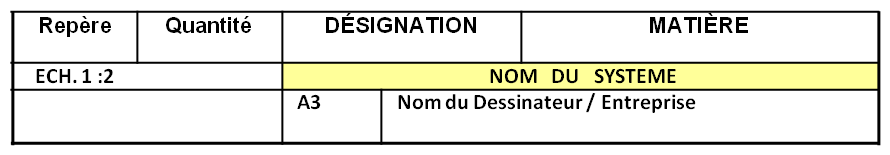
\includegraphics[width=0.9\linewidth]{img/Image6}
\end{minipage}

}}

{\frame{
\frametitle{La nomenclature}

La nomenclature est:
\begin{itemize}
 \item Liée à un dessin d'ensemble, elle dresse la liste complète de tous les éléments constitutifs du système dessiné,
 \item Chaque élément est répertorié, numéroté et tous les renseignements nécessaires le concernant sont indiqués.
\end{itemize}

\vfill

\begin{minipage}{0.27\linewidth}
 \centering 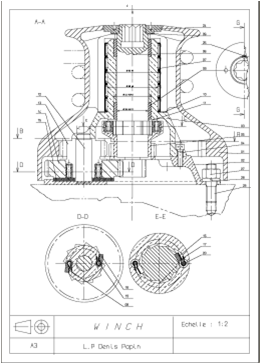
\includegraphics[width=\linewidth]{img/Image7}
\end{minipage}
\hfill
\begin{minipage}{0.27\linewidth}
 \centering 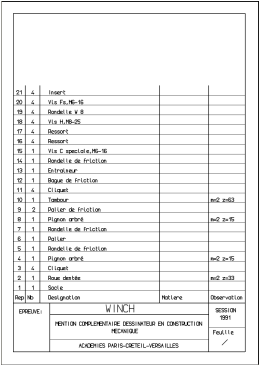
\includegraphics[width=\linewidth]{img/Image8}
\end{minipage}
\hfill
\begin{minipage}{0.4\linewidth}
 \centering 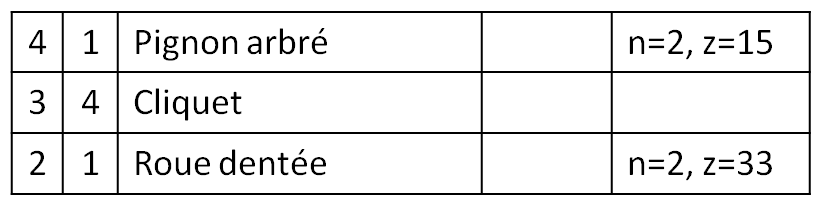
\includegraphics[width=\linewidth]{img/Image9}
\end{minipage}
}}

{\frame{
\frametitle{Les vues projetées}

\begin{minipage}{0.65\linewidth}
Les vues projetées sont nécessairement deux pour définir les caractéristiques géométriques d'un objet. Le nombre de 
vues devant être minimal afin d'aider la clarté du dessin, elles sont en général au maximum trois.

La vue de face est celle qui propose la meilleure définition de la pièce. Il est possible de lui associer quelques vues supplémentaires pour effacer toute 
ambiguïté :
\begin{itemize}
 \item Une pièce de révolution peut-être entièrement définie dans une vue axiale,
 \item Une pièce parallélépipédique nécessitera souvent 3 vues pour être définie en entier.
\end{itemize}
\end{minipage}
\hfill
\begin{minipage}{0.3\linewidth}
 \centering 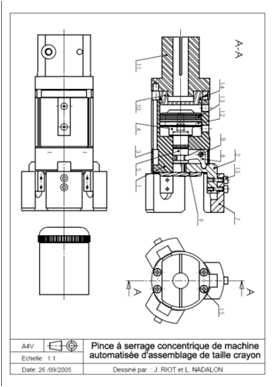
\includegraphics[width=\linewidth]{img/Image3}
\end{minipage}

}}

{\frame{
\frametitle{Les vues particulières}

\begin{itemize}
 \item La perspective
Elle donne des informations rapides sur les formes et l'organisation, elle ne permet pas de transmettre efficacement des données géométriques.
 \item La vue éclatée
Elle permet de faciliter l'identification, et l'emplacement des composants ainsi que des ordres d'assemblage pour l'atelier
 \item Les vues partielles
Elles permettent de représenter un détail à une échelle différente de celle choisie pour le dessin dans son ensemble.
\end{itemize}

\vfill

\begin{minipage}{0.4\linewidth}
 \centering 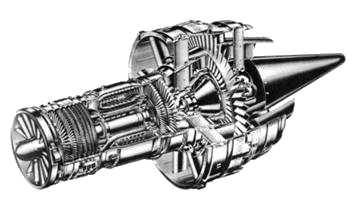
\includegraphics[width=\linewidth]{img/Image10}
\end{minipage}
\hfill
\begin{minipage}{0.4\linewidth}
 \centering 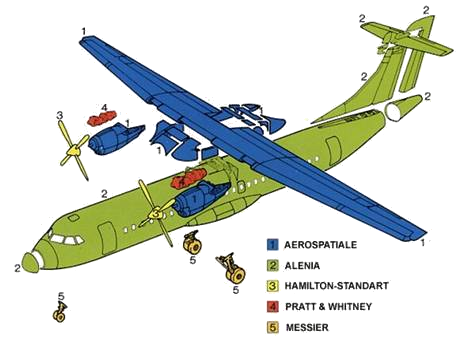
\includegraphics[width=\linewidth]{img/Image11}
\end{minipage}
}}

{\frame{
\frametitle{Correspondance des vues}

Il existe deux conventions pour placer les vues en correspondance, la représentation utilisée est indiquée par un cône tronqué placé dans le cartouche:
\begin{itemize}
 \item La convention européenne : la vue de dessus est placée sous la vue de face, la vue de droite, à gauche de la vue de face...
 \item La convention américaine : on place la vue de dessus au-dessus de la vue de face, la vue de gauche à sa gauche...
\end{itemize}

Règles de position relative des vues
\begin{itemize}
 \item Les projections d'un point sur les vues de face, gauche, droite, derrière sont situées sur une même ligne de rappel horizontal.
 \item Les projections d'un point sur les vues de face, dessus, dessous sont sur une même ligne de rappel vertical.
\end{itemize}

\vfill

 \centering 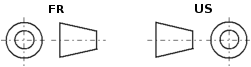
\includegraphics[width=0.4\linewidth]{img/Image12}
}}

{\frame{
\frametitle{Position relative des vues}

\ifdef{\public}{ \centering 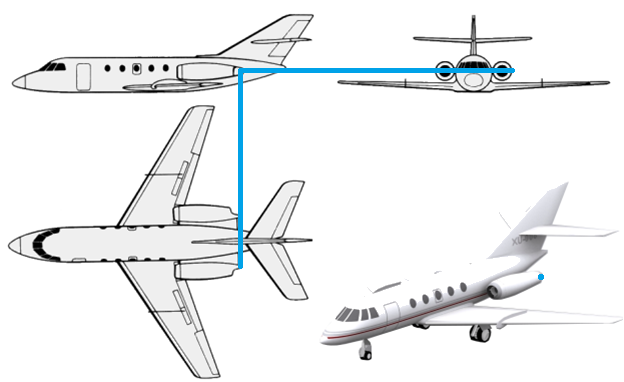
\includegraphics[width=0.9\linewidth]{img/Image13_cor}}{\centering 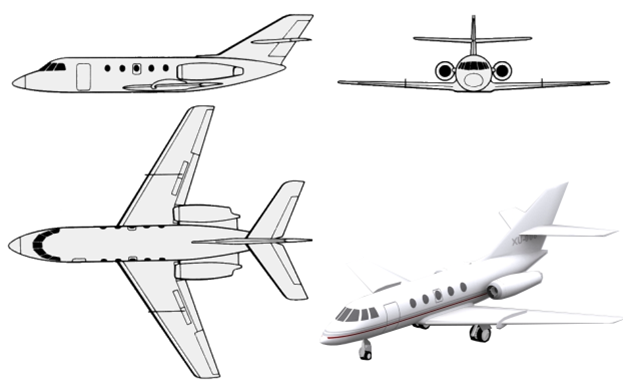
\includegraphics[width=0.9\linewidth]{img/Image13}}
}}

{\frame{
\frametitle{Les types de traits}

\begin{center}
\begin{tabular}{|cc|c|}
 \hline
 Type de trait & & Usages \\
 \hline
Continu fort & 
\includegraphics[width=3cm]{img/continu} & Arrêtes vives, visibles \\
 \hline
Interrompu (fin) & 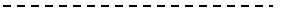
\includegraphics[width=3cm]{img/interrompu}& Arrêtes invisibles, pièces cachées \\
 \hline
Mixte fin & 
\includegraphics[width=3cm]{img/mixte}& Axes ou plans de symétrie \\
 \hline
Continu fin & 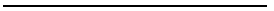
\includegraphics[width=3cm]{img/fin} & Arrêtes trangentes \\
 \hline
Continu fin à main levée & & Limites de coupe \\
 & 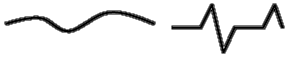
\includegraphics[width=3cm]{img/zigzag} & \\
 \hline
\end{tabular}
\end{center}
}}

{\frame{
\frametitle{Variateur Sandivar: Retrouvez les types de traits}

\centering 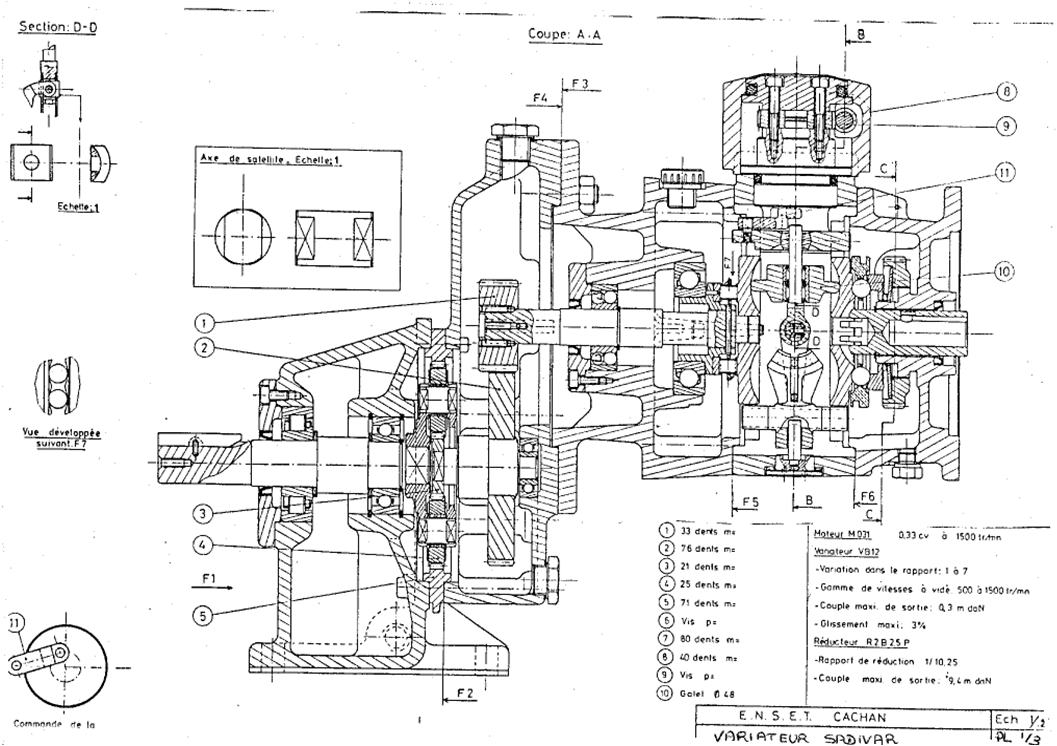
\includegraphics[width=0.85\linewidth]{img/Image14}
 
}}

{\frame{
\frametitle{La vue en coupe}

Les vues en coupe servent à la définition des formes cachées.

Convention :
\begin{itemize}
 \item La pièce centrale (qui n'a rien à cacher) ainsi que les pièces de révolution pleines (axes, vis, billes, écrou, clavettes ) ne sont pas coupées. 
 \item Les contours et arêtes vives sont en trait fort et la zone de la pièce coupée par le plan est hachurée en traits fins. 
 \item Les demi coupes sont utilisées pour des pièces symétriques, l'autre moitié est en vue extérieure.
 \item Les hachures indique le matériau de la pièce.
\end{itemize}

}}

{\frame{
\frametitle{Les sections}

\begin{minipage}{0.65\linewidth}
Les vues en coupe servent à la représentation des parties situées dans le plan de coupe.

Section sortie (Figure 1):
\begin{itemize}
 \item dessinée en trait fort pour tous les contours et en trait fin pour les hachures,
 \item placée dans le prolongement du plan de coupe ou dans le prolongement de l'axe de la pièce,
 \item les indications de coupes (plans, flèches, lettres) peuvent ne pas être placées s'il n'y a aucune ambiguïté possible.
\end{itemize}

Section rabattue (Figure 2):
\begin{itemize}
 \item rabattue directement sur la vue, dans ce cas elle se trace EN TRAIT FIN. Le plan de coupe et les flèches du sens d'observation sont facultatives.
\end{itemize}
\end{minipage}
\hfill
\begin{minipage}{0.3\linewidth}
\centering 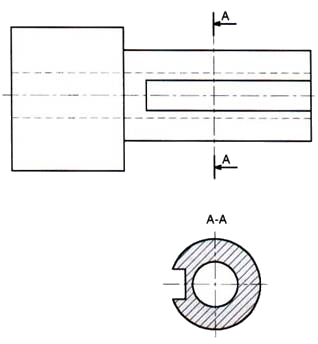
\includegraphics[width=0.85\linewidth]{img/Image15}

\centering 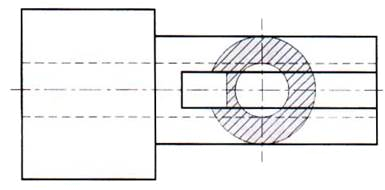
\includegraphics[width=0.85\linewidth]{img/Image16}
\end{minipage}
}}

{\frame{
\frametitle{Les hachures}

\begin{minipage}{0.7\linewidth}
Elles permettent une meilleure compréhension d'un dessin d'ensemble, et indiquent la nature des matériaux choisis par un motif.

Règles:
\begin{itemize}
 \item une même pièce doit avoir le même motif (orientation et fréquence) sur chaque vue,
 \item chaque pièce doit avoir une hachure différente,
 \item l'orientation des hachures entre deux pièces conjointes est alternée
 \item les pièces nervurées vues en coupe ne sont pas hachurées	
\end{itemize}
\end{minipage}
\hfill
\begin{minipage}{0.25\linewidth}
\centering 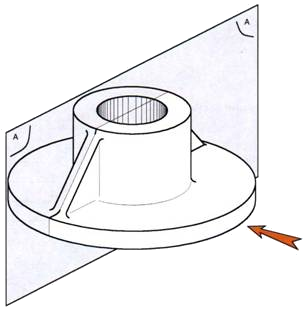
\includegraphics[width=0.85\linewidth]{img/Image17}

\centering 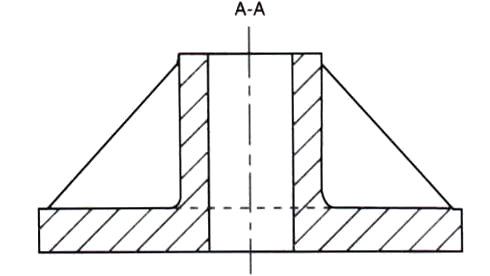
\includegraphics[width=0.85\linewidth]{img/Image18}
\end{minipage}

\vfill

\begin{center}
\begin{tabular}{|c|c|c|c|}
 \hline
 Acier & Aluminium & Alliage de cuivre & Matière plastique\\
   \ifdef{\public}{ \centering 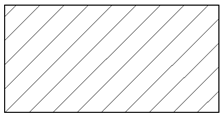
\includegraphics[width=2cm]{img/Image19}}{\centering 
\includegraphics[width=2cm]{img/Image19_vide}}
 & \ifdef{\public}{ \centering 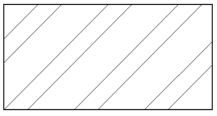
\includegraphics[width=2cm]{img/Image20}}{\centering 
\includegraphics[width=2cm]{img/Image19_vide}}
 & \ifdef{\public}{ \centering 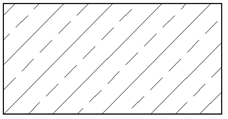
\includegraphics[width=2cm]{img/Image21}}{\centering 
\includegraphics[width=2cm]{img/Image19_vide}}
 & \ifdef{\public}{ 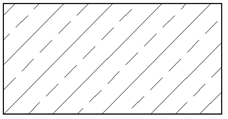
\includegraphics[width=2cm]{img/Image21}}{
\includegraphics[width=2cm]{img/Image19_vide}} \\
 \hline
\end{tabular}
\end{center}
}}

{\frame{
\frametitle{Vocabulaire des fonctions techniques}

\begin{minipage}{0.4\linewidth}
\begin{flushleft}
\ifdef{\public}{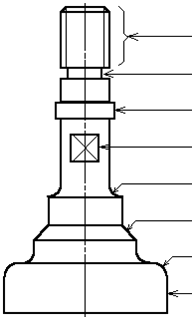
\includegraphics[width=0.6\linewidth]{img/Image25}}{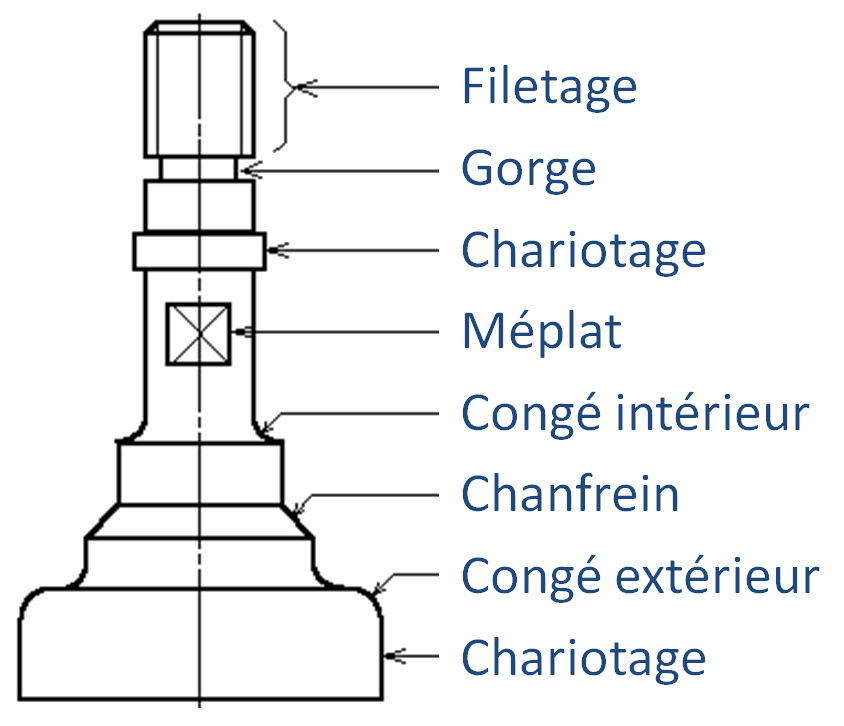
\includegraphics[width=\linewidth]{img/Image25_cor}}
\end{flushleft}
\end{minipage}
\hfill
\begin{minipage}{0.55\linewidth}
\centering 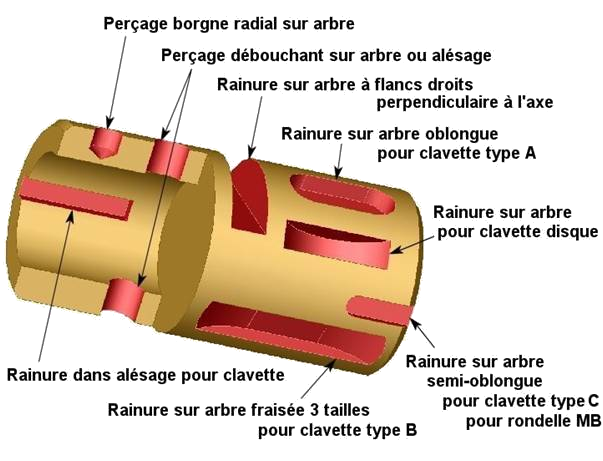
\includegraphics[width=0.7\linewidth]{img/Image23} \\
\centering 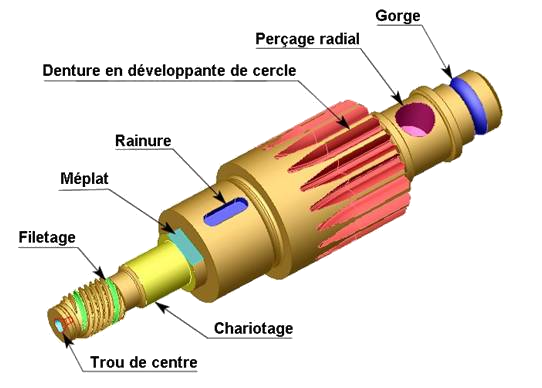
\includegraphics[width=0.7\linewidth]{img/Image24}
\end{minipage}
}}


{\frame{
\frametitle{Méthode de lecture de plan}

\begin{enumerate}
 \item Lire le Titre dans le cartouche
 \item Identifier l'organisation des vues (correspondance)
 \item Repérer les axes en traits mixtes (indiquent les directions des mouvements)
 \item Repérer les éléments standards (Vis, Roulements, engrenages, etc...)
\end{enumerate}

\centering 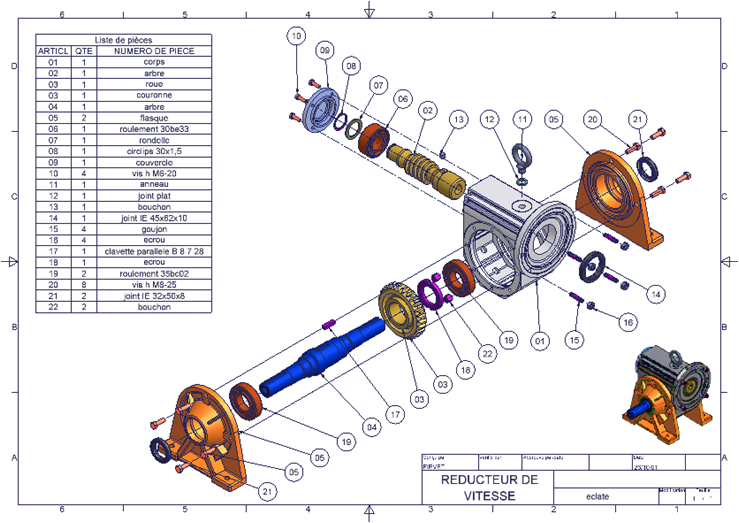
\includegraphics[width=0.6\linewidth]{img/Image26}
}}

{\frame{
\frametitle{La représentation d'un mécanisme}

\begin{savoir}
\begin{itemize}
 \item Vous devez être capables de lire le dessin technique d'un système afin d'en déduire le fonctionnement,
 \item Réaliser le schéma cinématique d'un système à partir de sa représentation sur un dessin technique,
 \item Représenter un système à l'aide des outils de représentation.
\end{itemize}
\end{savoir}

\begin{obj}
 \begin{itemize}
  \item Proposer des solutions de conception pour compléter la représentation d'un système,
  \item Compléter le dessin de définition d'un système en intégrant ces solutions.
 \end{itemize}
\end{obj}
}}


\end{document}
